\part{Automi e linguaggi}
\chapter{Linguaggi regolari}
\section{Automi finiti}

Il primo modello di calcolo studiato è quello degli automi a stati finiti (DFA - Deterministic Finite Automata). Si tratta di modelli semplici con memoria limitata. Sono spesso utilizzati per risolvere problemi concreti, come il riconoscimento di pattern.

\begin{Example}{Sensore di una porta automatica}{}
\textit{Il sistema di controllo per una porta automatica è un esempio di automa a stati finiti.} 

Una porta automatica ha un sensore davanti per rilevare la presenza di una persona che sta per attraversare la soglia. Un altro sensore è collocato dall'altro lato della soglia in modo che il sistema di controllo possa mantenere aperta la porta abbastanza a lungo da permettere alla persona di attraversarla e anche per evitare che la porta colpisca qualcuno che è dietro di essa quando si apre.

\begin{minipage}{\textwidth}
    \centering
    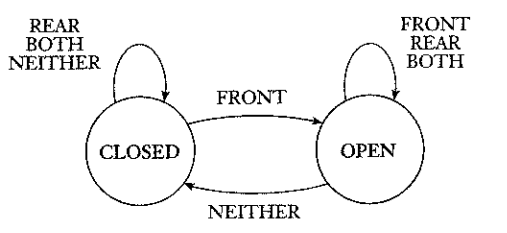
\includegraphics[width=0.5\textwidth]{images/porta-automatica.PNG}
    \captionof{figure}{Diagramma di stato per un sistema di controllo di una porta automatica}
\end{minipage}

Il sistema di controllo è in uno dei due stati: "OPEN" o "CLOSED," che rappresentano la condizione corrispondente della porta. Ci sono quattro possibili condizioni di input: "FRONT" (il cui significato è che una persona è sul sensore davanti alla soglia), "REAR" (significa che una persona è sul sensore dietro alla soglia), "BOTH" (significa che vi sono persone su entrambi i sensori), e "NEITHER" (significa che nessuno è su alcun sensore).

\begin{center}
    \begin{tabular}{|c|c|c|c|c|}
        \hline
        stato/input & \textbf{NEITHER} & \textbf{FRONT} & \textbf{REAR} & \textbf{BOTH} \\
        \hline
        \textbf{CLOSED} & CLOSED & OPEN & CLOSED & CLOSED \\
        \hline
        \textbf{OPEN} & CLOSED & OPEN & OPEN & OPEN \\
        \hline
    \end{tabular}
    \captionof{table}{Tabella delle transizioni di stato per il sistema di controllo di una porta automatica}
    \end{center}
\end{Example}

\begin{Definition}{Automa finito}{}
    In una prospettiva matematica, un DFA è definito come una tupla $(Q, \Sigma, \delta, q_0, F)$ dove:
    \begin{enumerate}
        \item $Q$ è un insieme finito chiamato insieme degli stati;
        \item $\Sigma$ è un insieme finito chiamato alfabeto di input;
        \item $\delta:Q\times\Sigma\to Q$ è la funzione di transizione;
        \item $q_0\in Q$ è lo stato iniziale;
        \item $F\subseteq Q$ è l'insieme degli stati finali o di accettazione.
    \end{enumerate}
    
    Il DFA accetta una stringa se, partendo dallo stato iniziale e seguendo le transizioni dettate dalla stringa, termina in uno stato finale.
\end{Definition}

\begin{figure}[ht]
    \centering
    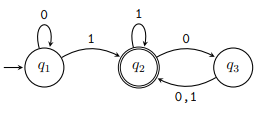
\includegraphics[width=0.4\linewidth]{images/automa-m1.PNG}
    \caption{Automa finito $M_1$}
    \label{fig:automa-m1}
\end{figure}

La Figura \ref{fig:automa-m1} mostra il diagramma di stato di un automa $M_1$. Esso ha tre stati, etichettati $q_{1}$, $q_2$ e $q_3$. Lo stato iniziale, $q_{1}$ è indicato dall'arco entrante in esso e non uscente da uno stato. Lo stato accettante, $q_{2}$, è quello con un doppio cerchio. Gli archi che vanno da uno stato a un altro sono chiamati transizioni.

Quando l'automa riceve una stringa in input esso elabora questa stringa e produce un output. L'elaborazione inizia nello stato iniziale di $M_1$. L'automa riceve i simboli della stringa di input uno a uno da sinistra a destra. Dopo aver letto ciascun simbolo, $M_1$ si muove da uno stato a un altro lungo la transizione che ha quel simbolo come etichetta. Quando legge l'ultimo simbolo, $M_1$ produce il suo output. L'output è "accetta" se $M_1$ è, in quel momento, in uno stato accettante e "rifiuta" se non lo è.

Possiamo descrivere $M_1$ formalmente ponendo $M_1=(Q, \Sigma, \delta, q_1, F)$ dove:
\begin{enumerate}
    \item $Q=\{q_1, q_2, q_3\}$;
    \item $\Sigma=\{0,1\}$;
    \item $d=$\begin{tabular}{c|c c}&0&1\\\hline $q_1$&$q_1$&$q_2$\\$q_2$&$q_3$&$q_2$\\$q_3$&$q_2$&$q_2$\\
    \end{tabular}
    \item $q_1$ è lo stato iniziale;
    \item $F=\{q_2\}$.
\end{enumerate}

Se $A$ è l'insieme di tutte le stringhe che la macchina $M$ accetta, diciamo che $A$ è il linguaggio della macchina $M$ e scriviamo $L(M) = A$. Diciamo che $M$ riconosce $A$ o che $M$ accetta $A$.

Una macchina può accettare diverse stringhe, ma riconosce sempre soltanto un linguaggio. Se la macchina non accetta alcuna stringa, essa riconosce ancora un linguaggio ossia, il linguaggio vuoto $\emptyset$. Nel nostro automa \ref{fig:automa-m1}, sia $A =\{x|x \textit{ contiene almeno un 1 e un numero pari di 0 segue l'ultimo 1}\}$, allora $L(M_{1}) = A$, o equivalentemente, $M_{1}$ riconosce $A$.

\begin{Example}{Automa finito $M_2$}{}
Ecco il diagramma di stato di un automa finito $M_2$:

\begin{minipage}{\textwidth}
    \centering
    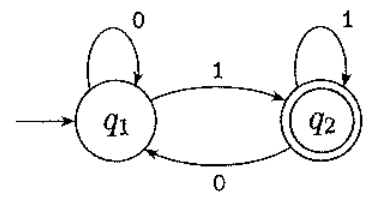
\includegraphics[width=0.3\textwidth]{images/automa-m2.PNG}
    \captionof{figure}{Diagramma di stato per un automa finito $M_2$}
\end{minipage}

Nella descrizione formale, $M_2$ è $(\{q_{1}, q_{2}\}, \{0, 1\}, \delta, q_{1}, \{q_{2}\})$. La funzione di transizione $\delta$ è: 
\begin{tabular}{c|c c}&0&1\\\hline $q_1$&$q_1$&$q_2$\\$q_2$&$q_1$&$q_2$\\
\end{tabular}. $M_{2}$ accetta tutte le stringhe che terminano con un 1. Quindi $L(M_{2}) =\{ w|w \textit{ termina con un 1}\}$.
\end{Example}

\subsection{Definizione formale di computazione}
Per definire il linguaggio associato di un automa si usa la funzione di transizione estesa: $\delta^*: Q\times\Sigma^*\to Q$\footnote{$\Sigma^*$ descrive il linguaggio che consiste di tutte le stringhe sull'alfabeto $\Sigma$.}, definita ricorsivamente come:
\begin{equation*}
\begin{cases}
    \delta^*(q, \epsilon) = \delta(q, \epsilon) = q&\textit{dove }\epsilon \textit{ rappresenta la stringa vuota}\\
    \delta^* (q, ax) = \delta^* (\delta(q, a), x)&\textit{dove } a \in \Sigma, x \in \Sigma^*
\end{cases}
\end{equation*}

Definiamo la coppia $(q, x)\in Q\times\Sigma^*$ come configurazione di un DFA che indica lo stato attuale e la parte ancora da leggere. 

Definiamo come passo di computazione la relazione binaria $\vdash_D$ definita come $(p, ax) \vdash_D (q, x) \iff \delta(p, a) = q$, dove $p, q\in Q$, $a\in\Sigma$ e $x\in\Sigma^*$. Posso estendere $\vdash_D$ a $\vdash_D^*$, ottenuta aggiungendo tutte le coppie in $Q\times\Sigma^*$ che rendono $\vdash_D$ chiusa per riflessività e transitività. In particolare la riflessività mi dice che $\forall q\in Q, x\in\Sigma^*, (q, x) \vdash_D^*(q, w)$, e la transitività mi dice che se $(q, abx) \vdash_D (p, bx) \land (p, bx) \vdash_D (r, x) \implies (q, abx) \vdash^*_D (r, y)$.

Sia $M = (Q, \Sigma, \delta, q_0, F)$ un automa finito e sia $w=w_1w_2...w_n$ una stringa dove ogni $w_i$ è un elemento dell'alfabeto $\Sigma$. Allora $M$ accetta $w$ se esiste una sequenza di stati $r_0, r_1,...,r_n$ in $Q$ con tre condizioni:
\begin{enumerate}
    \item $r_0=q_0$,
    \item $\delta(r_i ,w_{i + 1})=r_{i+1}$, \texttt{per i=0, ..., n-1}, e
    \item $r_n\in F$.
\end{enumerate}

La condizione 1 afferma che la macchina inizia nello stato iniziale. La condizione 2 afferma che la macchina passa da stato a stato in base alla funzione di transizione. La condizione 3 afferma che la macchina accetta il suo input se termina la lettura in uno stato accettante.


\begin{Definition}{Stringa accettata}{}
    Una stringa $x\in\Sigma^*$ è accettata da DFA se:
    \begin{equation*}
        \delta^*(q_0, x)\in F
    \end{equation*}
    Il linguaggio riconosciuto da $D$ è:
    \begin{equation*}
        L(D)=\{x\in\Sigma^*|\delta^*(q_0, x)\in F\}
    \end{equation*}
\end{Definition}

\begin{Definition}{Linguaggi regolari}{}
    Un linguaggio è definito regolare se:
    \begin{equation*}
        REG=\{L\subseteq\Sigma^*|\exists \textit{ DFA } D \textit{ t.c. } L(D)=L\}
    \end{equation*}
    ovvero se un automa finito lo riconosce.
\end{Definition}

\subsection{Progettare automi finiti}
\begin{Example}{Linguaggi regolari}{}
    \textit{Costruire un DFA per il linguaggio $L(D)=\{x\in\{0, 1\}^*|w_H(x)\geq3\}$.}

    \begin{minipage}{\textwidth}
        \centering
        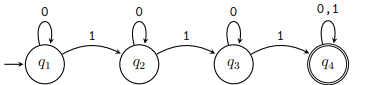
\includegraphics[width=0.5\textwidth]{images/es-linguaggi-regolari.PNG}
        %\captionof{figure}{Diagramma di stato per un automa finito $M_2$}
    \end{minipage}

    Se $x\in L$ allora $D$ accetta $x$, se $D$ accetta $x$ allora si ha $w_H(x)\geq3$.
\end{Example}

\begin{Example}{Linguaggi regolari}{}
    \textit{Costruire un DFA per il linguaggio $L(D)=\{x\in\{0, 1\}^*|x=1y \textit{ con }y\in\{0,1\}^*\}$.}

    \begin{minipage}{\textwidth}
        \centering
        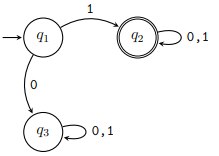
\includegraphics[width=0.3\textwidth]{images/es-linguaggi-regolari1.PNG}
        %\captionof{figure}{Diagramma di stato per un automa finito $M_2$}
    \end{minipage}
\end{Example}

\begin{Example}{Linguaggi regolari}{}
    \textit{Costruire un DFA per il linguaggio $L(D)=\{x\in\{0, 1\}^*|x=0^n1 \textit{ con }n\in\mathbb{N}-\{0\}\}$.}

    \begin{minipage}{\textwidth}
        \centering
        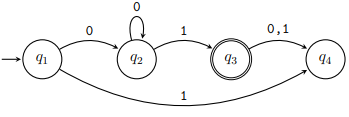
\includegraphics[width=0.5\textwidth]{images/es-linguaggi-regolari2.PNG}
        %\captionof{figure}{Diagramma di stato per un automa finito $M_2$}
    \end{minipage}
\end{Example}

\subsection{Le operazioni regolari}
Definiamo tre operazioni sui linguaggi, chiamate operazioni regolari, e le usiamo per studiare le proprietà dei linguaggi regolari.

\begin{Definition}{Operazione sui linguaggi}{}
    Dati i linguaggi $L, L_1, L_2 \subseteq \Sigma^*$, definiamo le seguenti operazioni:
    \begin{itemize}
        \item \textit{Operatore unione:} $L_1 \cup L_2 = \{x \in \Sigma^*| x \in L_1 \lor x \in L_2\}$;
        \item \textit{Operatore intersezione:} $L_1 \cap L_2 = \{x \in \Sigma^* | x \in L_1 \land x \in L_2\}$;
        \item \textit{Operatore complemento:} $\lnot L = \{x \in \Sigma^* | x \notin L\}$.
        \item \textit{Operatore concatenazione:} $L_1 \circ L_2 = \{xy \in \Sigma^*| x \in L_1, y \in L_2\}$

        L'operazione di concatenazione antepone una stringa di $L_1$ ad una stringa di $L_2$ in tutti i modi possibili per ottenere le stringhe nel nuovo linguaggio.
        \item \textit{Operatore potenza:} $L^n = \begin{cases}
            \{\epsilon\}&\textit{se } n = 0\\L\circ L^{n-1}&\textit{se } n > 0\end{cases}$
        \item \textit{Operatore star:} $L^* = {x_1 ... x_k \in \Sigma^*| k \geq 0, \forall i \in [1, k] x_i \in L} = \bigcup_{n\geq0} L^n$

        L'operazione star opera concatenando un numero qualsiasi di stringhe in $L$ insieme per ottenere una stringa nel nuovo linguaggio. Poiché "un numero qualsiasi" include 0 come possibilità, la stringa vuota e è sempre un elemento di $L^*$, indipendentemente da chi sia $L$.
    \end{itemize}
\end{Definition}

\begin{Example}{Operazione di concatenazione sui linguaggi}{}
    Siano $L_1=\{a, ab, ba\}$ e $L_2=\{ab, b\}$ allora:
    \begin{equation*}
        L_1\circ L_2 = \{aab, ab, abab, abb, baab, bab\}
    \end{equation*}
\end{Example}

\begin{Example}{Operazione di potenza sui linguaggi}{}
    Siano $L_1=\{a, ab, ba\}$ allora:
    \begin{equation*}
        L^2=\{aa, aab, aba, abab, abba, baa, baab, baba\}
    \end{equation*}
\end{Example}

\begin{Example}{Operazione star sui linguaggi}{}
    Sia $L=\{a, b\}$ allora:
    \begin{equation*}
        L^*=\{\epsilon, a, b, aa, ab, ba, bb, ...\}
    \end{equation*}
\end{Example}

In generale, una classe di oggetti è chiusa rispetto a un'operazione se l'applicazione di questa operazione a elementi della classe restituisce un oggetto ancora nella classe. 

\begin{Thm}{Chiusura rispetto all'unione}{}
    \textit{La classe dei linguaggi regolari è chiusa rispetto all'operazione di unione. In altre parole, se $A_{1}$ e $A_{2}$ sono linguaggi regolari, lo è anche $A_{1}\cup A_{2}$.}

    \begin{osservation}
    Poiché $A_{1}$ e $A_{2}$ sono regolari, sappiamo che un automa $M_{1}$ riconosce $A_{1}$ e un automa finito $M_{2}$ riconosce $A_{2}$. Per provare che $A_{1}\cup A_{2}$ è regolare, esibiamo un automa finito, $M$, che riconosce $A_{1}\cup A_{2}$. 

    Questa è una prova costruttiva. Costruiamo $M$ da $M_{1}$ ed $M_{2}$. Per riconoscere il linguaggio unione, la macchina $M$ deve accettare il suo input esattamente quando $M_{1}$ o $M_{2}$ lo accetterebbero.

    Come possiamo far sí che la macchina $M$ simuli $M_{1}$ ed $M_{2}$? Immagina che tu sia $M$. Come ricevi i simboli input, uno a uno, tu simuli sia $M_{1}$ che $M_{2}$ contemporaneamente. In questo modo, è necessario scorrere l'input solo una volta. Ma come puoi tenere traccia di entrambe le simulazioni con una memoria finita? Tutto quello che hai bisogno di ricordare è lo stato in cui ciascuna macchina sarebbe se avesse letto l'input fino a quel punto. Quindi, devi ricordare una coppia di stati. Quante possibili coppie ci sono? Se $M_{1}$ ha $k_{1}$ stati ed $M_{2}$ ha $k_{2}$ stati, il numero delle coppie di stati è il prodotto $k_{1}\times k_{2}$. Questo prodotto sarà il numero degli stati in $M$, uno per ogni coppia. Le transizioni di $M$ vanno da coppia a coppia, aggiornando lo stato corrente sia per la componente in $M_{1}$ che per quella in $M_{2}$. Gli stati accettanti di M sono quelle coppie tali che $M_1$ o $M_2$ è in uno stato accettante.
    \end{osservation}

    \begin{demonstration}
    Supponiamo che $M_{1}$ riconosca $A_{1}$ dove $M_{1} = (Q_{1}, \Sigma, \delta_{1}, q_{1}, F_{1})$ ed $M_{2}$ riconosca $A_{2}$ dove $M_{2} = (Q_{2}, \Sigma, \delta_{2}, q_{2}, F_{2})$. 

    Costruiamo $M$ che riconosce $A_{1}\cup A_{2}$ dove $M = (Q, \Sigma, \delta, q_{0}, F)$.
    \begin{enumerate}
        \item $Q=\{(r_{1}, r_{2})| r_1 \in Q_1 \land r_{2} \in Q_{2}\}$. Questo insieme è il prodotto cartesiano degli insiemi $Q_{1}$ e $Q_{2}$ ed è denotato con $Q_{1}\times Q_{2}$. E' l'insieme di tutte le coppie di stati, il primo in $Q_{1}$ e il secondo in $Q_{2}$.
        \item $\Sigma$, l'alfabeto, è lo stesso di $M_{1}$ ed $M_{2}$ (il teorema resta vero se hanno alfabeti diversi, $\Sigma_{1}$ e $\Sigma_{2}$).
        \item $\delta$, la funzione di transizione, è definita come segue. Per ogni $(r_{1}, r_{2}) \in Q$ e ogni $a \in \Sigma$ sia:
        \begin{equation*}
        \delta((r_{1}, r_{2}), a) = (\delta_{1}(r_{1}, a), \delta_{2}(r_{2}, a))        
        \end{equation*}
        Quindi $\delta$ riceve uno stato di $M$ (che in realtà è una coppia di stati, uno in $M_{1}$ e uno in $M_{2}$), con un simbolo di input, e restituisce lo stato successivo di $M$.
        \item $q_0$ è la coppia $(q_{1}, q_{2})$.
        \item $F$ è l'insieme delle coppie in cui l'uno o l'altro elemento è uno stato accettante di $M_{1}$ o $M_{2}$. Possiamo scriverlo come:
        \begin{equation*}
        F=\{(r_{1}, r_{2})|r_1 \in F_1 \lor r_2 \in F_2 \}
        \end{equation*}
        Questa espressione è uguale a $F=(F_{1}\times Q_{2})\cup(Q_1\times F_2)$.
    \end{enumerate}
    \end{demonstration}
\end{Thm}

\begin{Thm}{Chiusura rispetto alla concatenazione}{}
\textit{La classe dei linguaggi regolari è chiusa rispetto all'operazione di concatenazione. In altre parole, se $A_1$ e $A_2$ sono linguaggi regolari, allora lo è anche $A_1\circ A_2$.}

Per provare questo teorema, proviamo qualcosa di simile alla prova del caso dell'unione. Come prima, possiamo iniziare con gli automi finiti $M_1$ ed $M_2$ che riconoscono i linguaggi regolari $A_1$ e $A_2$. Ma ora, invece di costruire l'automa $M$ che accetta il suo input se $M_1$ o $M_2$ lo accetta, esso deve accettare se il suo input può essere diviso in due parti, tali che $M_1$ accetta la prima parte ed $M_2$ accetta la seconda parte. Il problema è che $M$ non sa dove dividere il suo input (cioè, dove finisce la prima parte e inizia la seconda). Per risolvere questo problema, introduciamo una nuova tecnica chiamata non determinismo.
\end{Thm}

\section{Non determinismo}
Il non determinismo è un concetto utile che ha avuto un grande impatto sulla teoria della computazione. Finora nella nostra discussione, ogni passo di una computazione seguiva univocamente dal passo precedente. In questo caso parliamo di computazione deterministica. In una macchina non deterministica, possono esistere diverse scelte per lo stato successivo in ogni punto.

Il non determinismo è una generalizzazione del determinismo, quindi ogni automa finito deterministico è automaticamente un automa finito non deterministico. Come mostra la Figura \ref{fig:automa-non-deterministico}, gli automi finiti non deterministici possono avere ulteriori caratteristiche.

\begin{figure}[ht]
    \centering
    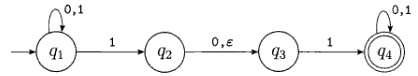
\includegraphics[width=0.5\linewidth]{images/automa-non-deterministico.png}
    \caption{Automa finito non deterministico}
    \label{fig:automa-non-deterministico}
\end{figure}

La differenza tra un automa finito deterministico, indicato con l'acronimo DFA, e un automa finito non deterministico, indicato con l'acronimo NFA, è subito evidente. In un NFA, uno stato può avere zero, uno, o più archi uscenti per ogni simbolo dell'alfabeto e, in generale, può avere archi etichettati con elementi dell'alfabeto o $\epsilon$.

Come computa un NFA? Supponiamo di eseguire un NFA su una stringa di input e di giungere in uno stato con più modi per procedere. La macchina si divide in più copie di sé stessa e segue tutte le possibilità in parallelo. Ogni copia della macchina prende una delle possibili direzioni per procedere. Se il simbolo di input successivo non compare su alcuno degli archi uscenti dallo stato occupato da una copia della macchina, quella copia della macchina "muore", insieme con il ramo della computazione a essa associato. Infine, se una qualunque di queste copie della macchina è in uno stato accettante alla fine dell'input, I'NFA accetta la stringa di input.

Un altro modo per considerare una computazione non deterministica è vederla come un albero di possibilità. La radice dell'albero corrisponde all'inizio della computazione. Ogni punto di ramificazione nell'albero corrisponde a un punto nella computazione in cui la macchina ha scelte multiple. La macchina accetta se almeno uno dei rami della computazione termina in uno stato accettante.

\begin{figure}[ht]
    \centering
    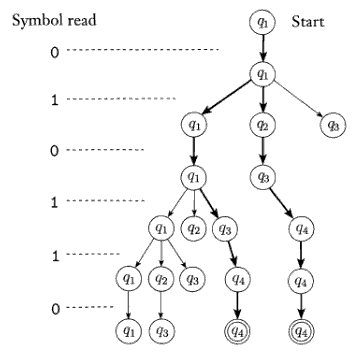
\includegraphics[width=0.5\linewidth]{images/automa-non-deterministico-input-010110.png}
    \caption{Computazione dell'automa \ref{fig:automa-non-deterministico} sull'input \texttt{010110}}
    \label{fig:automa-non-deterministico-input-010110}
\end{figure}

Nella descrizione formale, $N_{1}$ è $(Q, \Sigma, \delta, q_{1}, F)$ dove:
\begin{enumerate}
    \item $Q = \{q_{1}, q_{2}, q_{3}, q_{4}\}$,
    \item $\Sigma = \{0, 1\}$,
    \item $\delta$ è data da \begin{tabular}{c|ccc}&0&1&$\epsilon$\\\hline $q_1$&$\{q_1\}$&$\{q_1, q_2\}$&$\emptyset$\\$q_2$&$\{q_3\}$&$\emptyset$&$\{q_3\}$\\$q_3$&$\emptyset$&$\{q_4\}$&$\emptyset$\\$q_4$&$\{q_4\}$&$\{q_4\}$&$\emptyset$\\
\end{tabular}
    \item $q_{1}$ è lo stato iniziale, ed
    \item $F = \{q_{4}\}$.
\end{enumerate}


\begin{Example}{Automa non deterministico}{}
    \textit{Costruire un NFA che accetta le stringhe \texttt{$\epsilon$}, \texttt{a}, \texttt{baba}, e \texttt{baa}, ma che non accetta le stringhe \texttt{b}, \texttt{bb}, e \texttt{babba}.}

    \begin{minipage}{\textwidth}
        \centering
        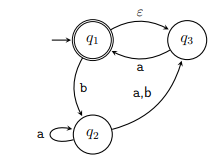
\includegraphics[width=0.3\textwidth]{images/esempio-automa-non-deterministico.PNG}
        %\captionof{figure}{Diagramma di stato per un automa finito $M_2$}
    \end{minipage}
\end{Example}

\subsection{Definizione formale di automa finito non deterministico}
\begin{Definition}{Automa finito non deterministico}{}
    Per un qualsiasi insieme $Q$ denotiamo con $\mathcal{P}(Q)$ la collezione di tutti i sottoinsiemi di $Q$. In questo caso $\mathcal{P}(Q)$ è chiamato l'insieme potenza di $Q$. Per ogni alfabeto $\Sigma$ scriviamo $\Sigma_\epsilon$ per denotare $\Sigma\cup\{\epsilon\}$. 
    
    Ora possiamo descrivere formalmente un automa finito non deterministico come una quintupla $(Q, \Sigma, \delta, q_{0}, F)$ dove:
    \begin{enumerate}
        \item $Q$ è un insieme finito di stati,
        \item $\Sigma$ è un alfabeto finito,
        \item $\delta: Q\times \Sigma_\epsilon\to\mathcal{P}(Q)$ è la funzione di transizione,
        \item $q_{0} \in Q$ è lo stato iniziale, ed
        \item $F\subseteq Q$ l'insieme degli stati di accettazione.
    \end{enumerate}    
\end{Definition}

Una configurazione per NFA $N$ è $(q, z)\in Q\times\Sigma^*_\epsilon$. Diremo $(p, ax)\vdash_N(q, x)\iff q\in S(p, a), a\in\Sigma_\epsilon, x\in\Sigma^*_\epsilon$. Posso considerare la chiusura simmetrica e transitiva di $\vdash_N$, detta $\vdash_N^*$. $N$ accetta $w\in\Sigma_\epsilon^*\iff\exists q\in F|(q_0, w)\vdash_N^*(q, \epsilon)$.

La definizione formale di computazione per un NFA è simile a quella per un DFA. Sia $N = (Q, \Sigma, \delta, q_{0}, F)$ un NFA e sia $w$ una stringa sull'alfabeto $\Sigma$. Diciamo che $N$ accetta $w$ se possiamo scrivere $w$ come $w= y_{1}y_{2} ... y_m$ , dove ciascun $y_{i}$ è un elemento di $\Sigma_{\epsilon}$ ed esiste una sequenza di stati $r_{0}, r_{1},...,r_m$ in $Q$ con tre condizioni:
\begin{enumerate}
    \item $r_{0} = q_{0}$
    \item $r_{i + 1} \in \delta(r_i ,y_{i+1})$, \texttt{for i=0, ..., m-1}, ed
    \item $r_{m} \in F$.
\end{enumerate}

La condizione 1 dice che la macchina inizia nello stato iniziale. La condizione 2 dice che lo stato $r_{i + 1}$ è uno dei possibili stati successivi quando $N$ è nello stato $r_{i}$ e sta leggendo $y_{i + 1}$. Osserva che $\delta(r_i ,y_{i + 1})$ è l'insieme dei possibili stati successivi e quindi diciamo che $r_{i + 1}$ è un elemento di quell'insieme. Infine, la condizione 3 dice che la macchina accetta il suo input se l'ultimo stato è uno stato accettante.

\subsection{Equivalenza tra gli NFA e i DFA}
Gli automi finiti deterministici e quelli non deterministici riconoscono la stessa classe di linguaggi.
Diciamo che due macchine sono equivalenti se esse riconoscono lo stesso linguaggio.

\begin{Thm}{Equivalenza tra gli NFA e i DFA}{}\label{thm:eq-nfa-dfa}
\textit{Per ogni automa finito non deterministico esiste un automa finito deterministico equivalente.}
\begin{osservation}
Se un linguaggio è riconosciuto da un NFA, allora dobbiamo mostrare l'esistenza di un DFA che lo riconosce. L'idea è trasformare l'NFA in un DFA equivalente che simula I'NFA.

Ricorda la strategia "lettore come automa" per progettare automi finiti. Come simuleresti l'NFA se stessi immaginando di essere un DFA? Cosa devi memorizzare dell'elaborazione della stringa di input? Se $k$ è il numero degli stati dell'NFA, esso ha $2 ^ k$ sottoinsiemi di stati. Ogni sottoinsieme corrisponde a una delle possibilità che il DFA deve ricordare, quindi il DFA che simula l'NFA avrà $2 ^ k$ stati.
\end{osservation}

\begin{demonstration}
Sia $N = (Q, \Sigma, \delta, q_{0}, F)$ l'NFA che riconosce un linguaggio $A$. Costruiamo un DFA $M = (Q', \Sigma, \delta', q_{0}', F')$ che riconosce $A$. Prima di fare la costruzione completa, consideriamo inizialmente il caso più semplice in cui $N$ non ha $\epsilon$-archi. In seguito considereremo gli $\epsilon$-archi.
\begin{enumerate}
    \item $Q' = \mathcal{P}(Q)$

    Ogni stato di $M$ è un insieme di stati di $N$. Ricorda che $\mathcal{P}(Q)$ è l'insieme dei sottoinsiemi di $Q$.
    \item Per $R \in Q'$ e $a \in \Sigma$ sia $\delta'(R,a)=\{q \in Q| q \in \delta(r, a) \textit{ per qualche } r \in R\}$.

    Se $R$ è uno stato di $M$, esso è anche un insieme di stati di $N$. Quando $M$ legge un simbolo $a$ nello stato $R$, mostra dove $a$ porta ogni stato in $R$. Poiché da ogni stato si può andare in un insieme di stati, prendiamo l'unione di tutti questi insiemi. Un altro modo per scrivere questa espressione è:
    \begin{equation*}
        \delta'(R,a)=\bigcup_{r \in R}\delta(r, a)
    \end{equation*}
    \item $q_{0}' = \{q_{0}\}$
    
    $M$ inizia nello stato corrispondente alla collezione che contiene solo lo stato iniziale di $N$.
    \item $F' =\{ R \in Q' |R \textit{ contiene uno stato accettante di } N\}$.

    La macchina $M$ accetta se uno dei possibili stati in cui $N$ potrebbe essere a quel punto è uno stato accettante.
\end{enumerate}

Ora dobbiamo considerare gli $\epsilon$-archi. Per farlo, introduciamo qualche ulteriore notazione. Per ogni stato $R$ di $M$, definiamo $E(R)$ come la collezione di stati che possono essere raggiunti dagli elementi di $R$ proseguendo solo con $\epsilon$-archi, includendo gli stessi elementi di $R$. Formalmente, per $R\subseteq Q$ sia:
\begin{equation*}
    E(R) =\{ q|q \textit{ può essere raggiunto da } R \textit{ attraverso } 0 \textit{ o più } \epsilon\textit{-archi}\}
\end{equation*}

Poi modifichiamo la funzione di transizione di $M$ seguendo tutti gli stati che possono essere raggiunti proseguendo attraverso $\epsilon$-archi dopo ogni passo. Sostituendo $\delta(r, a)$ con $E(\delta(r, a))$ realizziamo questo effetto. Quindi:
\begin{equation*}
    \delta'(R, a) = \{q \in Q | q \in E(\delta(r, a)) \textit{ per qualche } r \in R\}
\end{equation*}

Inoltre, dobbiamo modificare lo stato iniziale di $M$ per seguire tutti i possibili stati che possono essere raggiunti dallo stato iniziale di $N$ attraverso gli $\epsilon$-archi. Cambiare $q'_0$ in $E(\{q_{0}\})$ realizza questo risultato. Ora abbiamo completato la costruzione del DFA $M$ che simula I'NFA $N$.

Ovviamente la costruzione di $M$ funziona correttamente. A ogni passo nella computazione di $M$ su un input, chiaramente entra in uno stato che corrisponde al sottoinsieme di stati in cui $N$ potrebbe essere a quel punto. Quindi la nostra prova è completa.
\end{demonstration}  
\end{Thm}

\begin{Example}{Trasformare un NFA in un DFA}{}
Illustriamo la procedura che abbiamo dato nella prova del Teorema \ref{thm:eq-nfa-dfa} per trasformare un NFA in un DFA. 

\begin{minipage}{\textwidth}
    \centering
    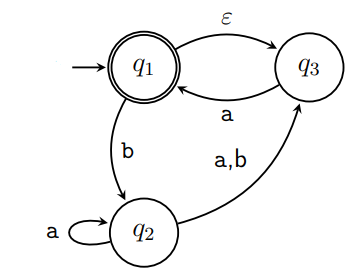
\includegraphics[width=0.3\textwidth]{images/eq-nfa-dfa.PNG}
    %\captionof{figure}{Diagramma di stato per un automa finito $M_2$}
\end{minipage}

Per costruire un DFA $D$ equivalente innanzitutto determiniamo gli stati di $D$. L'NFA ha tre stati quindi costruiamo $D$ con otto stati, uno per ogni sottoinsieme dell'insieme degli stati. 
\begin{equation*}
    \{\emptyset, \{q_1\}, \{q_2\}, \{q_3\}, \{q_1, q_2\}, \{q_2, q_3\}, \{q_1, q_3\}, \{q_1, q_2, q_3\}\}
\end{equation*}

Poi, determiniamo lo stato iniziale e gli stati accettanti di D. Lo stato iniziale è $E(\{q_1\})$ l'insieme degli stati che sono raggiungibili da $q_1$ passando attraverso $\epsilon$-archi, più $q_1$ stesso. Un $\epsilon$-arco va da $q_1$ a $q_3$, quindi $E(\{q_1\}) = \{q_1,q_3\}$. I nuovi stati accettanti sono quelli che contengono lo stato accettante dell'NFA quindi $\{\{q_1\}, \{q_1, q_2\}, \{q_1, q_3\}, \{q_1, q_2, q_3\}\}$. Infine, determiniamo la funzione di transizione di $D$. Ciascuno degli stati di $D$ va in una posizione sull'input $a$ e in una posizione sull'input $b$. Illustriamo il processo di determinare la posizione degli archi di transazione di D con pochi esempi.

In $D$, lo stato $\{q_2\}$ va in $\{q_2,q_3\}$ sull'input $a$ perché nell'NFA, lo stato $q_2$ va sia in $q_2$ che in $q_3$ sull'input $a$ e non possiamo andare più lontano da $q_2$ o $q_3$ attraverso $\epsilon$-archi. Lo stato $\{q_2\}$ va nello stato $\{q_3\}$ sull'input $b$ perché nell'NFA lo stato $q_2$ va solo nello stato $q_3$ sull'input $b$ e da $q_3$ non possiamo andare più lontano attraverso $\epsilon$-archi. Lo stato $\{q_1\}$ va in $\emptyset$ su $a$ perché nessun arco etichettato con $a$ esce da esso. Va in $\{q_2\}$ su $b$. Nota che la procedura nel Teorema \ref{thm:eq-nfa-dfa} specifica che seguiamo gli $\epsilon$-archi dopo ogni simbolo di input che viene letto. Una procedura alternativa basata sul seguire gli $\epsilon$-archi prima di leggere ogni simbolo funziona ugualmente bene.

Lo stato $\{q_3\}$ va in $\{q_1,q_3\}$ su $a$ perché nell'NFA, lo stato $q_3$ va in $q_1$ su $a$ e $q_1$ a sua volta va in $q_3$ con un $\epsilon$-arco. Lo stato $\{q_3\}$ su $b$ va in $\emptyset$.

Lo stato $\{q_1,q_2\}$ su $a$ va in $\{q_2,q_3\}$ perché $q_1$ non punta ad alcuno stato con $a$ archi, $q_2$ punta sia a $q_2$ che a $q_3$ con $a$ archi, e nessuno dei due punta altrove con $\epsilon$-archi. Lo stato $\{q_1,q_2\}$ su $b$ va in $\{q_2,q_3\}$. Continuando in questo modo, otteniamo il seguente diagramma per $D$.

\begin{minipage}{\textwidth}
    \centering
    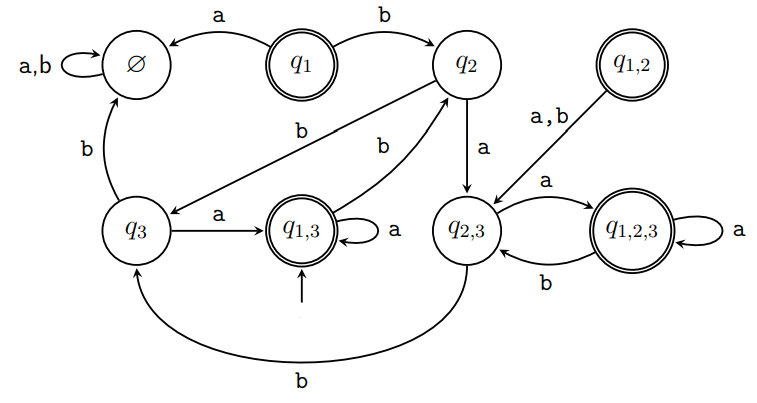
\includegraphics[width=0.6\textwidth]{images/eq-nfa-dfa2.PNG}
    %\captionof{figure}{Diagramma di stato per un automa finito $M_2$}
\end{minipage}
\end{Example}

\subsection{Chiusura rispetto alle operazioni regolari}
Ora torniamo alla chiusura della classe dei linguaggi regolari rispetto alle operazioni regolari. Il nostro scopo provare che l'unione, la concatenazione, e lo star di linguaggi regolari sono ancora regolari.

Innanzitutto, consideriamo di nuovo la chiusura rispetto all'unione. Prima abbiamo provato la chiusura rispetto all'unione simulando deterministicamente e simultaneamente entrambe le macchine, attraverso la costruzione di un prodotto cartesiano. Ora diamo una nuova prova per illustrare la tecnica del non determinismo.

\begin{Thm}{I linguaggi regolari sono chiusi rispetto all'unione}{}
    \textit{Abbiamo i linguaggi regolari $A_{1}$ e $A_{2}$ e vogliamo provare che $A_{1} \cup A_2$ è regolare.} 
    
    L'idea è prendere due NFA, $N_{1}$ ed $N_{2}$ per $A_{1}$ e $A_{2}$ e comporli in un nuovo NFA, $N$.

    La macchina $N$ deve accettare il suo input se $N_{1}$ o $N_2$ accetta questo input. La nuova macchina ha un nuovo stato iniziale che si dirama negli stati iniziali delle vecchie macchine con $\epsilon$-archi. In questo modo, la nuova macchina ipotizza non deterministicamente quale delle due macchine accetta l'input. Se una di esse accetta l'input, anche $N$ lo accetterà.

    Rappresentiamo questa costruzione nella figura seguente dove mostriamo come comporre $N_{1}$ ed $N_{2}$ in $N$ aggiungendo archi di transizione supplementari.

    \begin{minipage}{\textwidth}
        \centering
        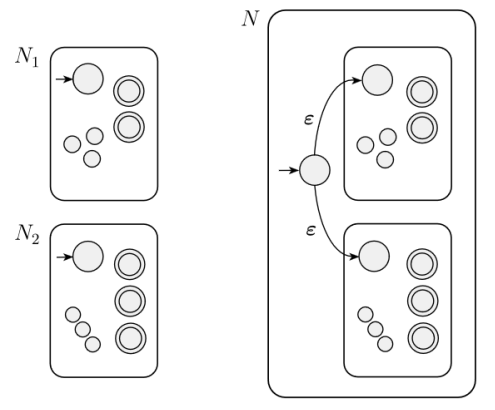
\includegraphics[width=0.4\textwidth]{images/costruzione-NFA-unione.png}
        %\captionof{figure}{Diagramma di stato per un automa finito $M_2$}
    \end{minipage}

    \begin{demonstration}
    Sia $N_{1} = (Q_{1}, \Sigma, \delta_{1}, q_{1}, F_{1})$ che riconosce $A_{1}$ ed $N_{2} = (Q_{2}, \Sigma, \delta_{2}, q_{2}, F_{2})$ che riconosce $A_{2}$.

    Costruiamo $N = (Q, \Sigma, \delta, q_{0}, F)$ per riconoscere $A_{1} \cup A_2$:
    \begin{enumerate}
        \item $Q= \{q_{0}\} \cup Q_1 \cup Q_2$.
        
        Gli stati di $N$ sono tutti gli stati di $N_{1}$ ed $N_{2}$ con l'aggiunta di un nuovo stato iniziale $q_{0}$.
        \item Lo stato $q_0$ è lo stato iniziale di $N$.
        \item L'insieme degli stati accettanti $F=F_1\cup F_2$. 
        
        Gli stati accettanti di $N$ sono tutti gli stati accettanti di $N_{1}$ ed $N_{2}$. In questo modo, $N$ accetta se $N_{1}$ accetta o $N_{2}$ accetta.
        \item Definiamo $\delta$ in modo che per ogni $q \in Q$ e ogni $a \in \Sigma_{\epsilon}$,
        \begin{equation*}
        \delta(q, a)=\begin{cases}
             \delta_1(q,a)&q \in Q_1 \\ \delta_2 (q,a)&q \in Q_2 \\\{q_1 ,q_2\}&q=q_0 \textit{ e } a=\epsilon\\ \emptyset&q=q_0 \textit{ e } a\neq\epsilon
        \end{cases}
        \end{equation*}
    \end{enumerate}
    \end{demonstration}
\end{Thm}

Ora possiamo provare la chiusura rispetto alla concatenazione.

\begin{Thm}{I linguaggi regolari sono chiusi rispetto alla concatenazione}{}
\textit{La classe dei linguaggi regolari è chiusa rispetto all'operazione di concatenazione.}

\begin{osservation}
Abbiamo i linguaggi regolari $A_{1}$ e $A_{2}$ vogliamo provare che $A_{1}\circ A_2$ è regolare. L'idea è prendere due NFA, $N_{1}$ ed $N_{2}$ per $A_{1}$ ed $A_{2}$ e combinarli in un nuovo NFA $N$ come abbiamo fatto nel caso dell'unione, ma questa volta in un modo diverso.

\begin{minipage}{\textwidth}
    \centering
    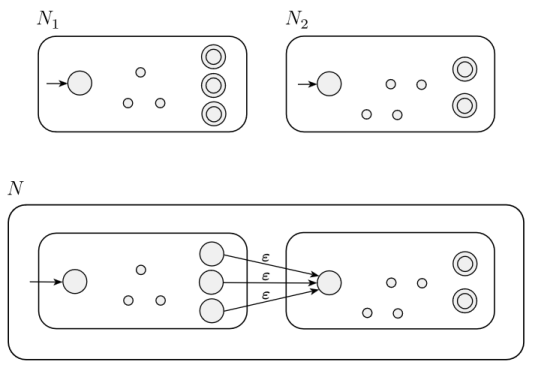
\includegraphics[width=0.5\textwidth]{images/costruzione-NFA-concatenazione.png}
    %\captionof{figure}{Diagramma di stato per un automa finito $M_2$}
\end{minipage}

Poniamo come stato iniziale di $N$ lo stato iniziale di $N_{1}$. Gli stati accettanti di $N_{1}$ hanno degli ulteriori $\epsilon$-archi che non deterministicamente permettono di diramarsi in $N_{2}$ ogni volta che $N_{1}$ è in uno stato accettante, indicando che ha trovato un pezzo iniziale dell'input che costituisce una stringa in $A_{1}$. Gli stati accettanti di $N$ sono solo gli stati accettanti di $N_{2}$. Quindi esso accetta quando l'input può essere diviso in due parti, la prima accettata da $N_{1}$ e la seconda da $N_{2}$. Possiamo pensare che $N$ non deterministicamente ipotizza dove effettuare la divisione.
\end{osservation}

\begin{demonstration}
Sia $N_{1} = (Q_{1}, \Sigma, \delta_{1}, q_{1}, F_{1})$ che riconosce $A_{1}$ ed $N_{2} = (Q_{2}, \Sigma, \delta_{2}, q_{2}, F_{2})$ che riconosce $A_{2}$.

Costruiamo $N = (Q, \Sigma, \delta, q_{1}, F_{2})$ per riconoscere $A_{1}\circ A_2$.
\begin{enumerate}
    \item $Q =Q_1\cup Q_2$.
    
    Gli stati di $N$ sono tutti gli stati di $N_{1}$ ed $N_{2}$.
    \item Lo stato $q_{1}$ è uguale allo stato iniziale di $N_{1}$.
    \item Gli stati accettanti $F_{2}$ sono uguali agli stati accettanti di $N_{2}$.
    \item Definiamo $\delta$ in modo che per ogni $q \in Q$ e ogni $a \in \Sigma_{\epsilon}$,
    \begin{equation*}
    \delta(q,a)=\begin{cases}
        \delta_1(q,a)&q\in Q_1 \textit{ e }q \notin F_1\\ \delta_1(q,a)&q \in F_1\textit{ e }a \neq\epsilon\\ \delta_1(q,a)\cup\{q_2\}& q \in F_{1} \textit{ e }a = \epsilon \\ \delta_2(q,a)&q \in Q_2
    \end{cases}
    \end{equation*}
\end{enumerate}
\end{demonstration}
\end{Thm}

\begin{Thm}{I linguaggi regolari sono chiusi rispetto all'operazione star}{}
\textit{La classe dei linguaggi regolari è chiusa rispetto all'operazione star.}

\begin{osservation}
Abbiamo un linguaggio regolare $A_{1}$ e vogliamo provare che anche $A_{1}^*$ è regolare. Prendiamo un NFA $N_{1}$ per $A_{1}$ e lo modifichiamo per riconoscere $A_{1}^*$. L'NFA $N$ risultante accetterà il suo input quando esso può essere diviso in varie parti ed $N_{1}$ accetta ogni parte.

Possiamo costruire $N$ come $N_{1}$ con $\epsilon$-archi supplementari che dagli stati accettanti ritornano allo stato iniziale. In questo modo, quando l'elaborazione giunge alla fine di una parte che $N_{1}$ accetta, la macchina $N$ ha la scelta di tornare indietro allo stato iniziale per provare a leggere un'altra parte che $N_{1}$ accetta. Inoltre, dobbiamo modificare $N$ in modo che accetti $\epsilon$, che è sempre un elemento di $A_{1}^*$. Un'idea (leggermente cattiva) è semplicemente aggiungere lo stato iniziale all'insieme degli stati accettanti. Questa strategia certamente aggiunge $\epsilon$ al linguaggio riconosciuto, ma può anche aggiungere altre stringhe non volute. Il modo per correggerla è aggiungere un nuovo stato iniziale, che è anche uno stato accettante, e che ha un $\epsilon$-arco entrante nel vecchio stato iniziale. Questa soluzione ha l'effetto desiderato di aggiungere $\epsilon$ al linguaggio senza aggiungere qualcos'altro.
\end{osservation}

\begin{minipage}{\textwidth}
    \centering
    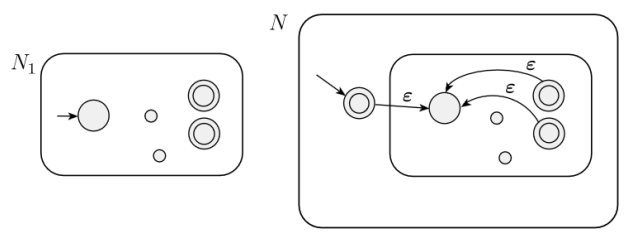
\includegraphics[width=0.6\textwidth]{images/costruzione-NFA-star.png}
    %\captionof{figure}{Diagramma di stato per un automa finito $M_2$}
\end{minipage}

\begin{demonstration}
Sia $N_{1} = (Q_{1}, \Sigma, \delta_{1}, q_{1}, F_{1})$ che riconosce $A_{1}$. Costruiamo $N = (Q, \Sigma, \delta, q_{0}, F)$ per riconoscere $A_{1}^*$.

\begin{enumerate}
    \item $Q=\{q_{0}\}\cup Q_1$.

    Gli stati di $N$ sono gli stati di $N_{1}$ più un nuovo stato iniziale.

    \item Lo stato $q_0$ è il nuovo stato iniziale.
    \item $F=\{q_{0}\} \cup F_1$

    Gli stati accettanti sono i vecchi stati accettanti più il nuovo stato iniziale.

    \item Definiamo $\delta$ in modo che per ogni $q \in Q$ e ogni $a \in \Sigma_{\epsilon}$,
    \begin{equation*}
    \delta(q,a)=\begin{cases}
        \delta_1(q,a)&q\in Q_1 \textit{ e }q \notin F_1\\ \delta_1(q,a)&q \in F_1\textit{ e }a \neq\epsilon\\ \delta_1(q,a)\cup\{q_1\}& q \in F_{1} \textit{ e }a = \epsilon \\ \{q_1\}&q=q_0 \textit{ e } a=\epsilon\\ \emptyset&q=q_0\textit{ e } a\neq\epsilon
    \end{cases}
    \end{equation*}
\end{enumerate}
\end{demonstration}
\end{Thm}

\section{Espressioni regolari}
Analogamente alle espressioni algebriche, possiamo usare le operazioni regolari per costruire espressioni che descrivono linguaggi, che sono chiamate espressioni regolari. Un esempio è $(0\cup 1)0^*$.

Il valore di un'espressione regolare è un linguaggio. In questo caso, il valore è il linguaggio che consiste di tutte le stringhe che iniziano con uno 0 o un 1 seguito da un qualsiasi numero di simboli uguali a 0. Otteniamo questo risultato dividendo l'espressione nelle sue parti. In primo luogo, i simboli 0 e 1 sono abbreviazioni per gli insiemi $\{0\}$ e $\{1\}$. Quindi $(0\cup 1)$ significa $(\{0\} \cup\{1\})$. Il valore di questa parte è il linguaggio $\{0, 1\}$. La parte $0^*$ denota $\{0\}^*$, e il suo valore è il linguaggio che consiste di tutte le stringhe contenenti un numero qualsiasi di simboli uguali a 0. Inoltre, come il simbolo $\times$ in algebra, il simbolo della concatenazione $\circ$ è spesso sottinteso nelle espressioni regolari. Quindi $(0\cup 1)0^*$ è in realtà un'abbreviazione per $(0\cup 1)\circ 0^*$. La concatenazione connette le stringhe dalle due parti per ottenere il valore dell'intera espressione.

Le espressioni regolari hanno un ruolo importante nelle applicazioni dell'informatica. Nelle applicazioni che coinvolgono testo, gli utenti possono voler cercare stringhe che soddisfano alcuni schemi. Le espressioni regolari forniscono un metodo potente per descrivere tali schemi.

Nelle espressioni regolari, l'operazione star è eseguita per prima, seguita dalla concatenazione e infine dall'unione, a meno che delle parentesi non cambino l'ordine usuale.

\begin{Definition}{Espressione regolare}{}
Diciamo che $R$ è un'espressione regolare se $R$ è
\begin{enumerate}
    \item $a$ per qualche $a$ nell'alfabeto $\Sigma$,
    \item $\epsilon$,
    \item $\emptyset$,
    \item $(R_{1}\cup R_2)$ dove $R_{1}$ ed $R_{2}$ sono espressioni regolari,
    \item $(R_{1}\circ R_2)$ dove $R_{1}$ ed $R_{2}$ sono espressioni regolari, o
    \item $(R_{1}^*)$ dove $R_{1}$ è un'espressione regolare.
\end{enumerate}

Nei punti 1 e 2, le espressioni regolari $a$ e $\epsilon$ rappresentano i linguaggi $\{a\}$ e $\{\epsilon\}$, rispettivamente. Nel punto 3, l'espressione regolare $\emptyset$ rappresenta il linguaggio vuoto. Nei punti 4, 5, e 6, le espressioni rappresentano i linguaggi ottenuti prendendo l'unione o la concatenazione dei linguaggi $R_{1}$ ed $R_{2}$ o lo star del linguaggio $R_{1}$ rispettivamente.
\end{Definition}

Non confondere le espressioni regolari $\epsilon$ e $\emptyset$. L'espressione $\epsilon$ rappresenta il linguaggio che contiene una sola stringa ossia, la stringa vuota - mentre $\emptyset$ rappresenta il linguaggio che non contiene alcuna stringa.

Apparentemente, sembra che stiamo definendo la nozione di espressione regolare in termini di sé stessa. Se fosse vero, avremmo una definizione circolare, che non sarebbe valida. Comunque, $R_{1}$ ed $R_{2}$ sono sempre più piccole di $R$. Quindi in realtà stiamo definendo le espressioni regolari in termini di espressioni regolari più piccole, evitando in tal modo la circolarità. Una definizione di questo tipo è chiamata una definizione induttiva.

\begin{Example}{Espressioni regolari}{}
Negli esempi seguenti, assumiamo che l'alfabeto $\Sigma$ sia $\{0,1\}$.
\begin{enumerate}
    \item $0^*10^* = \{w|w \textit{ contiene un solo } 1\}$.
    \item $\Sigma^*1\Sigma^* = \{w|w\textit{ ha almeno un }1\}$.
    \item $\Sigma^*001\Sigma^* = \{w|w\textit{ contiene la stringa }001\textit{ come sottostringa}\}$.
    \item $(0\cup \epsilon)(1 \cup \epsilon)= \{\epsilon, 0, 1, 01\}$
    \item $1^*\emptyset=\emptyset$.
        
    Concatenando l'insieme vuoto a un qualsiasi insieme si ottiene l'insieme vuoto.
    \item $\emptyset^* = \{\epsilon\}$

    L'operazione star concatena un numero qualsiasi di stringhe del linguaggio per ottenere una stringa nel risultato. Se il linguaggio è vuoto, l'operazione star può concatenare 0 stringhe, dando solo la stringa vuota.
\end{enumerate}
\end{Example}

\subsection{Equivalenza con gli automi finiti}
Le espressioni regolari e gli automi finiti sono equivalenti rispetto alla loro potenza descrittiva. Ogni espressione regolare può essere trasformata in un automa finito che riconosce il linguaggio che essa descrive, e viceversa. Ricorda che un linguaggio regolare è un linguaggio che è riconosciuto da qualche automa finito.

\begin{Thm}{Linguaggio ed espressione regolare}{}\label{thm:ling-espr-reg}
\textit{Un linguaggio è regolare se e solo se qualche espressione regolare lo descrive.}
\end{Thm}

Questo teorema deve essere dimostrato in entrambe le direzioni. Noi enunciamo e proviamo ciascuna direzione in un lemma separato.

\begin{Lemma}{Espressione regolare implica linguaggio regolare}{}
\textit{Se un linguaggio è descritto da un'espressione regolare, allora esso è regolare.}

\begin{osservation}
Supponiamo di avere un'espressione regolare $R$ che descrive un linguaggio $A$. Mostriamo come trasformare $R$ in un NFA che riconosce $A$. Se un NFA riconosce $A$ allora $A$ è regolare.
\end{osservation}

\begin{demonstration}
Trasformiamo $R$ in un NFA $N$. Consideriamo i sei casi nella definizione di espressione regolare.
\begin{enumerate}
    \item $R=a$ per qualche $a\in\Sigma$. Allora $L(R)=\{a\}$ e il seguente NFA riconosce $L(R)$.

    \begin{minipage}{\textwidth}
    \centering
    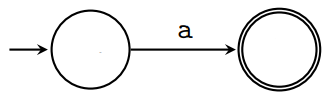
\includegraphics[width=0.25\textwidth]{images/lemma-ling-espr1.PNG}
    %\captionof{figure}{Diagramma di stato per un automa finito $M_2$}
    \end{minipage}
    
    Formalmente, $N= (\{q_1,q_2\}, \Sigma, \delta, q_1, \{q_2\})$, dove descriviamo $\delta$ dicendo che $\delta(q_1,a) = \{q_2\}$ e $\delta(r,b) = \emptyset$ per $r\neq q_1$ o $b\neq a$.

    \item $R=\epsilon$. Allora $L(R) = \{\epsilon\}$ e il seguente NFA riconosce $L(R)$.

    \begin{minipage}{\textwidth}
    \centering
    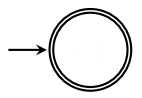
\includegraphics[width=0.1\textwidth]{images/lemma-ling-espr2.PNG}
    %\captionof{figure}{Diagramma di stato per un automa finito $M_2$}
    \end{minipage}
    
    Formalmente, $N= (\{q_1\}, \Sigma, \delta, q_1, \{q_1\})$, dove $\delta(r,b) = \emptyset$ per ogni $r$ e $b$. 
    
    \item $R=\emptyset$. Allora $L(R)=\emptyset$, e il seguente NFA riconosce $L(R)$.

    \begin{minipage}{\textwidth}
    \centering
    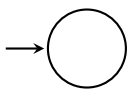
\includegraphics[width=0.1\textwidth]{images/lemma-ling-espr3.PNG}
    %\captionof{figure}{Diagramma di stato per un automa finito $M_2$}
    \end{minipage}

    Formalmente, $N= (\{q\}, \Sigma, \delta, q, \emptyset)$, dove $\delta(r, b) = \emptyset$ per ogni $r$ e $b$.

    \item $R=R_1\cup R_2$.
    \item $R=R_1\circ R_2$.
    \item $R=R_1^*$.
\end{enumerate}

Per gli ultimi tre casi, usiamo le costruzioni date nelle prove che la classe dei linguaggi regolari è chiusa rispetto alle operazioni regolari. In altre parole, costruiamo l'NFA per $R$ dagli NFA per $R_1$ ed $R_2$ (o solo $R_1$ nel caso 6) e mediante l'appropriata costruzione della chiusura.
\end{demonstration}
\end{Lemma}

Questo termina la prima parte della prova del Teorema \ref{thm:ling-espr-reg}, dando la direzione più facile della condizione "se e solo se".

\begin{Definition}{Automa finito non deterministico generalizzato}{}
Un automa finito non deterministico generalizzato è una quintupla, $(Q,\Sigma, \delta, q_{start}, q_{accept})$, dove
\begin{enumerate}
    \item $Q$ è l'insieme finito degli stati,
    \item $\Sigma$ è l'alfabeto di input,
    \item $\delta:(Q - \{q_{accept}\})\times (Q-\{q_{start}\}) \longrightarrow \mathcal{R}$ è la funzione di transazione,
    \item $q_{start}$ è lo stato iniziale e
    \item $q_{accept}$ è lo stato accettante.
\end{enumerate}
\end{Definition}

Gli automi finiti non deterministici generalizzati sono semplicemente automi finiti non deterministici nei quali gli archi delle transizioni possono avere espressioni regolari come etichette, invece che solo elementi dell'alfabeto o $\epsilon$. Il GNFA legge blocchi di simboli dall'input, non necessariamente solo un simbolo alla volta come in un comune NFA. Il GNFA si muove lungo un arco di transizione che collega due stati leggendo un blocco di simboli dall'input che formano una stringa descritta dall'espressione regolare su quell'arco. Un GNFA è non deterministico e quindi può avere diversi modi di elaborare la stessa stringa di input. Esso accetta il suo input se la sua elaborazione può far si che il GNFA sia in uno stato accettante alla fine dell'input.

Un GNFA accetta una stringa $w$ in $\Sigma^*$ se $w= w_{1}w_{2}...w_k$ dove ogni $w_{i}$ è in $\Sigma^*$ ed esiste una sequenza di stati tale che $q_{0}, q_{1},..., q_k$ tale che
\begin{enumerate}
    \item $q_{0}=q_{start}$ è lo stato iniziale,
    \item $q_{k}=q_{accept}$ lo stato accettante e
    \item per ogni $i$, risulta $w_{i} \in L(R_{i})$ dove $R_i = \delta(q_{i - 1}, q_i)$; in altre parole, $R_{i}$ è l'espressione sull'arco da $q_{i-1}$ a $q_i$.
\end{enumerate}

\begin{Lemma}{Linguaggio regolare implica espressione regolare}{}
\textit{Se un linguaggio è regolare, allora è descritto da un'espressione regolare.}

\begin{osservation}
Dobbiamo mostrare che se un linguaggio $A$ è regolare, allora un'espressione regolare lo descrive. Poiché $A$ è regolare, esso è accettato da un DFA. Descriviamo una procedura per trasformare i DFA in espressioni regolari equivalenti.    
\end{osservation}

Dividiamo questa procedura in due parti, usando un nuovo tipo di automa finito chiamato automa finito non deterministico generalizzato, GNFA. Prima mostriamo come trasformare un DFA in un GNFA e poi come trasformare un GNFA in un'espressione regolare.

Per comodità, richiediamo che i GNFA abbiano sempre una forma speciale che soddisfi le seguenti condizioni.
\begin{itemize}
    \item Lo stato iniziale ha archi di transizione uscenti verso un qualsiasi altro stato ma nessun arco entrante proveniente da un qualsiasi altro stato.
    \item Esiste un solo stato accettante, ed esso ha archi entranti provenienti da un qualsiasi altro stato ma nessun arco uscente verso un qualsiasi altro stato. Inoltre, lo stato accettante non è uguale allo stato iniziale.
    \item Eccetto che per lo stato iniziale e lo stato accettante, un arco va da ogni stato ad ogni altro stato e anche da ogni stato in sé stesso.
\end{itemize}

Possiamo facilmente trasformare un DFA in un GNFA nella forma speciale. Aggiungiamo semplicemente un nuovo stato iniziale con un $\epsilon$-arco che entra nel vecchio stato iniziale e un nuovo stato accettante con $\epsilon$-archi entranti, provenienti dai vecchi stati accettanti. Se alcuni archi hanno più etichette (o se ci sono più archi che collegano gli stessi due stati nella stessa direzione), sostituiamo ognuno di essi con un solo arco la cui etichetta è l'unione delle precedenti etichette. Infine, aggiungiamo archi con etichetta $\emptyset$ tra stati che non hanno archi. Questo ultimo passo non cambierebbe il linguaggio riconosciuto perché una transizione etichettata con $\emptyset$ non può mai essere usata. Da qui in poi assumiamo che tutti i GNFA sono nella forma speciale.

Ora mostriamo come trasformare un GNFA in un'espressione regolare. Supponiamo che il GNFA abbia $k$ stati. Allora, poiché un GNFA deve avere uno stato iniziale e uno stato accettante ed essi devono essere diversi tra loro, sappiamo che $k\geq 2$. Se $k > 2$, costruiamo un GNFA equivalente con $k-1$ stati. Questo passo può essere ripetuto sul nuovo GNFA fino a quando esso è ridotto a due stati. Se $k=2$, il GNFA ha un solo arco che va dallo stato iniziale allo stato accettante. L'etichetta di questo arco è l'espressione regolare equivalente.

Il passo cruciale è costruire un GNFA equivalente con uno stato in meno quando $k > 2$. Lo facciamo scegliendo uno stato, estraendolo dalla macchina, e modificando il resto in modo che sia ancora riconosciuto lo stesso linguaggio. Ogni stato può essere scelto, purché non sia lo stato iniziale o lo stato accettante. Siamo certi che un tale stato esiste perché $k > 2$. Chiamiamo $q_{rip}$ lo stato rimosso.

Dopo aver rimosso $q_{rip}$ modifichiamo la macchina cambiando le espressioni regolari che etichettano ciascuno dei restanti archi. Le nuove etichette controbilanciano l'assenza di $q_{rip}$ reintegrando le computazioni perse. La nuova etichetta che va da uno stato $q_{i}$ a uno stato $q_{j}$ è un'espressione regolare che descrive tutte le stringhe che porterebbero la macchina da $q_{i}$ a $q_{j}$ o direttamente o tramite $q_{rip}$. Illustriamo questa strategia:

\begin{minipage}{\textwidth}
\centering
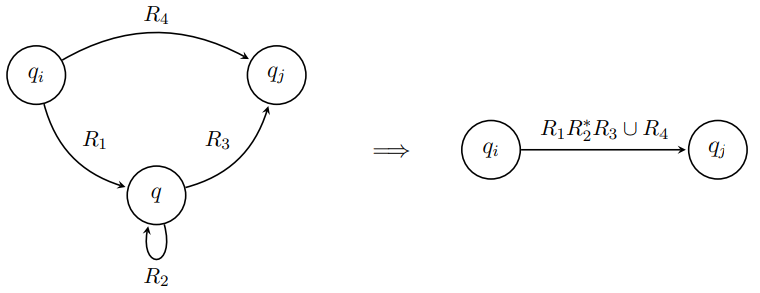
\includegraphics[width=0.7\textwidth]{images/GFA-stato-in-meno.PNG}
%\captionof{figure}{Diagramma di stato per un automa finito $M_2$}
\end{minipage}

Nella vecchia macchina, se
\begin{enumerate}
    \item $q_{i}$ va a $q_{rip}$ con un arco etichettato $R_{1}$,
    \item $q_{rip}$ va in sé stesso con un arco etichettato $R_{2}$,
    \item $q_{rip}$ va a $q_{j}$ con un arco etichettato $R_{3}$,
    \item $q_{i}$ va a $q_{j}$ con un arco etichettato $R_{4}$,
\end{enumerate}

allora nella nuova macchina, l'arco da $q_{i}$ a $q_{j}$ riceve l'etichetta
\begin{equation*}
    (R_{1}) (R_2)^*(R_3)\cup(R_4)
\end{equation*}

Facciamo questa modifica per ogni arco che va da un qualsiasi stato $q_{i}$ a un qualsiasi stato $q_{j}$ includendo il caso in cui $q_{i} = q_{j}$. La nuova macchina riconosce il linguaggio di partenza.

\begin{demonstration}
Formalizziamo questa idea. In primo luogo, per rendere più facile la prova, definiamo formalmente il nuovo tipo di automa introdotto. Un GNFA è simile a un automa finito non deterministico tranne che per la funzione di transizione, che ha la forma
\begin{equation*}
    \delta: (Q-\{q_{accept}\}) \times (Q-\{q_{start}\})\longrightarrow \mathcal{R}
\end{equation*}

Il simbolo $\mathcal{R}$ è la collezione di tutte le espressioni regolari sull'alfabeto $\Sigma$, e $q_{start}$ e $q_{accept}$ sono gli stati iniziale e accettante. Se $\delta (q_i, q_j) = \mathcal{R}$, l'arco dallo stato $q_i$ allo stato $q_j$ ha come etichetta l'espressione regolare $\mathcal{R}$. Il dominio della funzione di transizione è $(Q-\{q_{accept}\}) \times (Q-\{q_{start}\})$ perché un arco collega ogni stato a un qualsiasi altro stato, tranne che nessun arco è uscente da $q_{accept}$ o è entrante in $q_{start}$.

Sia $M$ il DFA per il linguaggio $A$. Allora trasformiamo $M$ in un GNFA $G$ aggiungendo un nuovo stato iniziale e un nuovo stato accettante e i necessari archi di transizione supplementari. Usiamo la procedura \texttt{CONVERT(G)} (vedi Algoritmo \ref{alg:convert}).
\end{demonstration}
\end{Lemma}

\begin{Algoritmo}{\texttt{CONVERT(G)}}{}\label{alg:convert}
\texttt{CONVERT(G)} prende un GNFA e restituisce un'espressione regolare equivalente. Questa procedura usa la ricorsione, che significa che essa chiama sé stessa. Evitiamo un ciclo infinito perché la procedura chiama sé stessa solo per elaborare un GNFA che ha uno stato in meno. Il caso in cui il GNFA ha due stati è trattato senza ricorsione.

\begin{enumerate}
    \item Sia $k$ il numero di stati di $G$.
    \item Se $k = 2$, allora $G$ deve consistere di uno stato iniziale, uno stato accettante, e un singolo arco che li collega ed è etichettato con un'espressione regolare $\mathcal{R}$. Restituisce l'espressione $\mathcal{R}$.
    \item Se $k > 2$ scegliamo un qualsiasi stato $q_{rip} \in Q$ diverso da $q_{start}$ e $q_{accept}$ e sia $G'$ il GNFA $(Q',\Sigma, \delta', q_{start}, q_{accept})$, dove 
    \begin{equation*}
        Q'=Q-\{q_{rip}\}
    \end{equation*} 
    e per ogni $q_i \in Q' -\{q_{accept}\}$ e ogni $q_j \in Q'-\{q_{start}\}$ poniamo 
    \begin{equation*}
        \delta'(q_{i}, q_{j})=(R_1)(R_2)^*(R_3)\cup(R_4)    
    \end{equation*}
    dove $R_1 = \delta(q_{i}, q_{rip})$, $R_2=\delta(q_{rip}, q_{rip})$, $R_3 = \delta(q_{rip}, q_j)$ ed $R_{4} = \delta(q_{i}, q_{j})$.
    \item Calcola \texttt{CONVERT(G')} e restituisce questo valore.
\end{enumerate}
\end{Algoritmo}

\begin{Thm}{\texttt{CONVERT(G)} è equivalente al GNFA}{}
\textit{Per ogni GNFA $G$, \texttt{CONVERT(G)} è equivalente a $G$.}

Proviamo quest'affermazione per induzione su $k$, il numero di stati del GNFA.

\begin{demonstration}\phantom{}

\begin{itemize}
    \item \textit{Passo base:} Proviamo che l'affermazione è vera per $k = 2$ stati. Se $G$ ha solo due stati, esso può avere solo un singolo arco, che va dallo stato iniziale allo stato accettante. L'espressione regolare che è l'etichetta di quest'arco descrive tutte le stringhe che permettono a $G$ di raggiungere lo stato accettante. Quindi quest'espressione è equivalente a $G$.
    \item \textit{Passo induttivo:} Assumiamo che l'affermazione sia vera per $k - 1$ stati e usiamo questa ipotesi per provare che l'affermazione è vera per $k$ stati. In primo luogo mostriamo che $G$ e $G'$ riconoscono lo stesso linguaggio. Supponiamo che $G$ accetti un input $w$. Allora in un ramo accettante della computazione, $G$ entra in una sequenza di stati:
    \begin{equation*}
        q_{start},q_1,q_2,q_3,...,q_{accept}
    \end{equation*}
    Se nessuno di essi è lo stato rimosso $q_{rip}$, evidentemente anche $G'$ accetta $w$. La ragione è che ciascuna delle nuove espressioni regolari che etichettano gli archi di $G'$ contiene le vecchie espressioni regolari come parte di un'unione. Se $q_{rip}$ è presente, eliminando ogni sequenza di stati $q_{rip}$ consecutivi creiamo una computazione accettante per $G'$. Gli stati $q_{i}$ e $q_{j}$ che raggruppano una tale sequenza hanno una nuova espressione sull'arco tra essi, la quale descrive tutte le stringhe che portano da $q_i$ a $q_j$, attraverso $q_{rip}$ in $G$. Quindi $G'$ accetta $w$.

    Viceversa, supponiamo che $G'$ accetti un input $w$. Poiché ciascun arco tra due qualsiasi stati $q_i$ e $q_j$ in $G'$ descrive la collezione delle stringhe che portano da $q_i$ a $q_j$ in $G$, o direttamente o attraverso $q_{rip}$, anche $G$ deve accettare $w$. Quindi $G$ e $G'$ sono equivalenti.
\end{itemize}

L'ipotesi induttiva afferma che quando l'algoritmo chiama sé stesso ricorsivamente sull'input $G$, il risultato è un'espressione regolare che è equivalente a $G'$ perché $G'$ ha $k-1$ stati. Quindi anche questa espressione regolare è equivalente a $G$, e abbiamo provato che l'algoritmo è corretto.
\end{demonstration}
\end{Thm}

\begin{Example}{Espressione regolare in NFA}{}
\textit{Trasformiamo l'espressione regolare $(a\cup ab)^*$ in un NFA.}

\begin{minipage}{\textwidth}
    \centering
    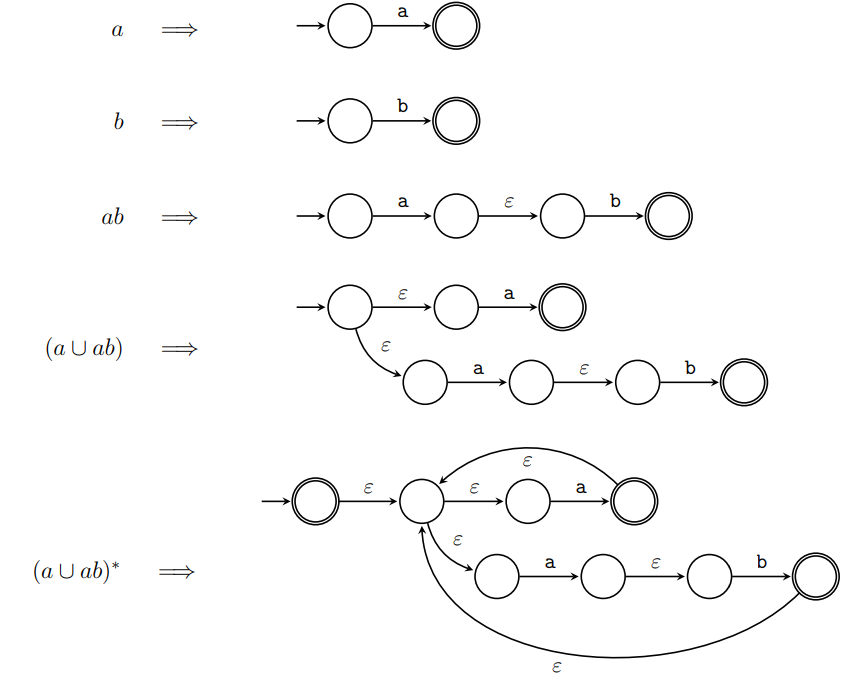
\includegraphics[width=0.8\textwidth]{images/esp-reg-in-nfa.PNG}
    %\captionof{figure}{Diagramma di stato per un automa finito $M_2$}
\end{minipage}
\end{Example}

\begin{Example}{Conversione DFA in espressione regolare}{}
\textit{Consideriamo il seguente DFA:}

\begin{minipage}{\textwidth}
    \centering
    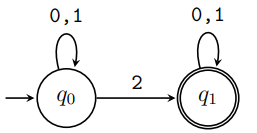
\includegraphics[width=0.25\textwidth]{images/dfa-esp-reg.PNG}
    %\captionof{figure}{Diagramma di stato per un automa finito $M_2$}
\end{minipage}
Il suo GNFA equivalente corrisponde a:

\begin{minipage}{\textwidth}
    \centering
    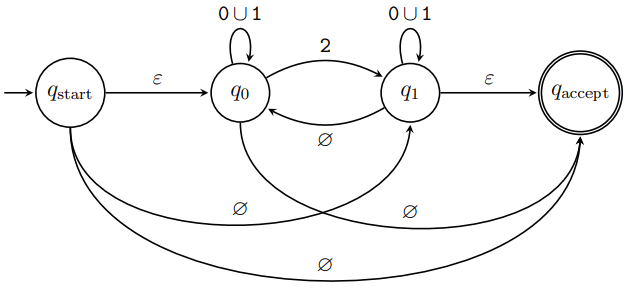
\includegraphics[width=0.6\textwidth]{images/gfna-esp-reg.PNG}
    %\captionof{figure}{Diagramma di stato per un automa finito $M_2$}
\end{minipage}

Rimuoviamo quindi lo stato $q_0$ calcolando le nuove transizioni:
\begin{gather*}
\delta'(q_{start}, q_1) = \delta(q_{start}, q_0)\delta(q_0, q_0)^*\delta(q_0, q_1) \cup \delta(q_{start}, q_1) = \epsilon(0 \cup 1)^*2 \cup \emptyset = (0 \cup 1)^*2\\
\delta'(q_{start}, q_{accept}) = \delta(q_{start}, q_0)\delta(q_0, q_0)^*\delta(q_0, q_{accept}) \cup \delta(q_{start}, q_{accept}) = \epsilon(0 \cup 1)^*\emptyset\cup\emptyset = \emptyset\\
\delta'(q_1, q_1) = \delta(q_1, q_0)\delta(q_0, q_0)^*\delta(q_0, q_1) \cup \delta(q_1, q_1) = \emptyset(0 \cup 1)^*2 \cup (0 \cup 1) = 0 \cup 1\\
\delta'(q_1, q_{accept}) = \delta(q_1, q_0)\delta(q_0, q_0)^*\delta(q_0, q_{accept}) \cup \delta(q_1, q_{accept}) = \emptyset(0 \cup 1)^*\emptyset \cup \epsilon = \epsilon\\
\end{gather*}

\begin{minipage}{\textwidth}
    \centering
    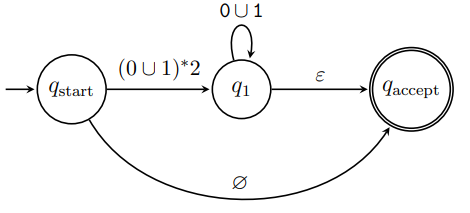
\includegraphics[width=0.45\textwidth]{images/gfna2-esp-reg.PNG}
    %\captionof{figure}{Diagramma di stato per un automa finito $M_2$}
\end{minipage}

Infine, rimuoviamo lo stato $q_1$ calcolando le nuove transizioni:
\begin{align*}
\delta''(q_{start}, q_{accept}) = \delta'(q_{start}, q_1)\delta'(q_1, q_1)^*\delta'(q_1, q_{accept}) \cup \delta'(q_{start}, q_{accept}) =\\ (0 \cup 1)^*2(0 \cup 1)^*\epsilon \cup \emptyset = (0 \cup 1)^*2(0 \cup 1)^*    
\end{align*}

Il GNFA minimale, dunque, corrisponde a:

\begin{minipage}{\textwidth}
    \centering
    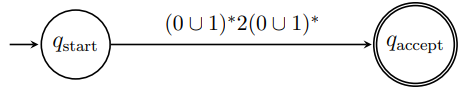
\includegraphics[width=0.45\textwidth]{images/gfna3-esp-reg.PNG}
    %\captionof{figure}{Diagramma di stato per un automa finito $M_2$}
\end{minipage}
\end{Example}

\section{Linguaggi non regolari}
Per comprendere il potere computazionale degli automi finiti dobbiamo anche comprenderne i limiti. In questa sezione, mostriamo come provare che alcuni linguaggi non possono essere riconosciuti da alcun automa finito.

Consideriamo il linguaggio $B=\{0^n1^n|n\geq0\}$ Se cerchiamo di trovare un DFA che riconosca $B$, scopriamo che la macchina sembra aver bisogno di ricordare quanti simboli uguali a 0 ha visto fin quando legge l'input. Poiché il numero di simboli uguali a 0 non è limitato, la macchina dovrà tenere traccia di un numero infinito di possibilità. Ma non può farlo con un numero finito di stati.

Di seguito presentiamo un metodo per provare che linguaggi come $B$ non sono regolari.

\subsection{Il pumping lemma per i linguaggi regolari}
La nostra tecnica per provare la non regolarità deriva da un teorema sui linguaggi regolari, tradizionalmente chiamato il pumping lemma. Questo teorema afferma che tutti i linguaggi regolari hanno una proprietà speciale. Se noi possiamo mostrare che un linguaggio non ha questa proprietà, siamo sicuri che esso non è regolare. La proprietà afferma che tutte le stringhe nel linguaggio possono essere "replicate" se la loro lunghezza raggiunge almeno uno specifico valore speciale, chiamato la lunghezza del pumping. Questo significa che ogni tale stringa contiene una parte che può essere ripetuta un numero qualsiasi di volte ottenendo una stringa che appartiene ancora al linguaggio.

\begin{Thm}{Pumping lemma}{}
\textit{Se $A$ è un linguaggio regolare, allora esiste un numero $p$ (la lunghezza del pumping) tale che se $s$ è una qualsiasi stringa in $A$ di lunghezza almeno $p$, allora $s$ può essere divisa in tre parti, $s = xyz$ soddisfacenti le seguenti condizioni:}
\begin{enumerate}
    \item per ogni $i \geq 0, xy^iz \in A$,
    \item $|y|>0$, e
    \item $|xy|\leq p$
\end{enumerate}

Ricordiamo che $|s|$ rappresenta la lunghezza della stringa $s$, $y^i$ indica $i$ copie di $y$ concatenate insieme, e $y ^ 0$ è uguale a $\epsilon$.

Quando $s$ è divisa in $xyz$, $x$ o $z$ potrebbe essere $\epsilon$, ma la condizione 2 dice che $y\neq\epsilon$. Osserva che senza la condizione 2 il teorema sarebbe banalmente vero. La condizione 3 afferma che le parti $x$ e $y$ insieme hanno lunghezza al più $p$. E' una condizione tecnica supplementare che ogni tanto troviamo utile quando dimostriamo che alcuni linguaggi non sono regolari.

\begin{osservation}
Sia $M = (Q, \Sigma, \delta, q_{1}, F)$ un DFA che riconosce $A$. Assegniamo alla lunghezza del pumping $p$ il numero degli stati di $M$. Mostriamo che ogni stringa $s$ in $A$ di lunghezza almeno $p$ può essere divisa nelle tre parti $xyz$, soddisfacenti le nostre tre condizioni. Cosa accade se nessuna stringa in $A$ è di lunghezza almeno $p$? Allora il nostro compito è perfino più facile perché il teorema diventa banalmente vero: ovviamente le tre condizioni valgono per tutte le stringhe di lunghezza almeno $p$ se non vi è alcuna di tali stringhe.

Se $s$ in $A$ ha lunghezza almeno $p$, consideriamo la sequenza di stati che $M$ attraversa nella computazione con input $s$. Inizia con lo stato iniziale $q_{1}$ poi va per esempio in $q_{3}$ poi per esempio in $q_{20}$ poi in $q_9$, e così via, finché raggiunge la fine di $s$ nello stato $q_{13}$. Se $s$ è in $A$, sappiamo che $M$ accetta $s$, quindi $q_{13}$ è uno stato accettante.

Se supponiamo che $n$ sia la lunghezza di $s$, la sequenza di stati $q_{1}, q_{3}, q_{20}, q_{9} ,...,q_{13}$ ha lunghezza $n + 1$. Poiché $n$ è almeno $p$, sappiamo $n + 1$ è più grande di $p$, il numero di stati di $M$. Quindi, la sequenza deve contenere uno stato che si ripete. Questo risultato è un esempio del principio della piccionaia, un nome di fantasia per il fatto piuttosto ovvio che se $p$ piccioni sono messi in una piccionaia con meno di $p$ nicchie, qualche nicchia deve avere più di un piccione in essa. Lo stato $q_9$ è quello che si ripete.

Ora dividiamo $s$ nelle tre componenti $x$, $y$ e $z$. La componente $x$ è la parte di $s$ che compare prima di $q_9$, la componente $y$ è la parte tra le due occorrenze di $q_9$ e la componente $z$ è la parte restante di $s$, che viene dopo la seconda occorrenza di $q_9$. Quindi $x$ porta $M$ dallo stato $q_1$ a $q_9$, $y$ riporta $M$ da $q_9$ a $q_9$ e $z$ porta $M$ da $q_9$ allo stato accettante $q_{13}$.

\begin{minipage}{\textwidth}
    \centering
    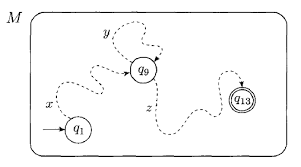
\includegraphics[width=0.5\textwidth]{images/linguaggi-non-regolari.png}
    %\captionof{figure}{Diagramma di stato per un automa finito $M_2$}
\end{minipage}

Vediamo perché questa divisione di $s$ soddisfa le tre condizioni. Supponiamo di eseguire $M$ sull'input $xyyz$. Sappiamo che $x$ porta $M$ da $q_1$ a $q_9$, e poi il primo $y$ lo riporta da $q_9$ a $q_9$, come fa il secondo $y$ e poi $z$ lo porta in $q_{13}$. Essendo $q_{13}$ uno stato accettante, $M$ accetta l'input $xyyz$. Analogamente, esso accetterà $xy^iz$ per ogni $i > 0$. Nel caso $i = 0$, $xy^iz=xz$, che è accettata per ragioni analoghe. Questo prova la condizione 1.

Per verificare la condizione 2, vediamo che $|y| > 0$, poiché era la parte di $s$ tra due diverse occorrenze dello stato $q_9$.

Per ottenere la condizione 3, ci assicuriamo che $q_9$ sia la prima ripetizione nella sequenza. Per il principio della piccionaia, i primi $p + 1$ stati nella sequenza devono contenere una ripetizione. Quindi, $|xy| \leq p$.
\end{osservation}

\begin{demonstration}
Sia $M = (Q, \Sigma, \delta, q_1, F)$ un DFA che riconosce $A$ e sia $p$ il numero di stati di $M$.

Sia $s=s_1s_2...s_n$ una stringa in $A$ di lunghezza $n$, dove $n\geq p$. Sia $r_1 ,...,r{n + 1}$ la sequenza di stati attraversati da $M$ mentre elabora $s$, quindi $r_{i + 1} = \delta(r_i ,s_i )$ per $1 \leq i \leq n$. Questa sequenza ha lunghezza $n + 1$ che è almeno $p + 1$. Due tra i primi $p + 1$ elementi nella sequenza devono essere lo stesso stato, per il principio della piccionaia. Chiamiamo il primo di questi $r_j$ e il secondo $r_l$. Poiché $r_l$ si presenta tra le prime $p + 1$ posizioni in una sequenza che inizia in $r_1$, abbiamo $l \leq p + 1$. Ora sia $x=s_1...s_{j-1}$, $y=s_j...s_{l-1}$ e $z=s_l...s_n$.

Poiché $x$ porta $M$ da $r_1$ a $r_j$, $y$ porta $M$ da $r_j$ a $r_j$ e $z$ porta $M$ da $r_j$ a $r_{n + 1}$ che è uno stato accettante, $M$ deve accettare $xy^iz$ per $i \geq 0$. Sappiamo che $j \neq l$, perciò $|y| > 0$, e $l\leq p + 1$, perciò $|xy|\leq p$. Quindi tutte le condizioni del pumping lemma sono rispettate.
\end{demonstration}
\end{Thm}

Per usare il pumping lemma per provare che un linguaggio $B$ non è regolare, in primo luogo si assuma che $B$ sia regolare per ottenere una contraddizione. Poi si usi il pumping lemma per assicurare l'esistenza di una lunghezza del pumping $p$ tale che tutte le stringhe di lunghezza maggiore o uguale a $p$ in $B$ possano essere iterate. In seguito, si trovi una stringa $s$ in $B$ che ha lunghezza maggiore o uguale a $p$, ma che non può essere iterata. Infine, si dimostri che $s$ non può essere iterata considerando tutti i modi di dividere $s$ in $x$, $y$ e $z$ (prendendo in considerazione la condizione 3 del pumping lemma se è utile) e, per ogni tale divisione, trovando un valore i tale che $xy^iz\notin B$. Questo passo finale spesso comporta il dover raggruppare i vari modi di dividere $s$ in diversi casi e l'analizzarli individualmente. L'esistenza di $s$ contraddirebbe il pumping lemma se $B$ fosse regolare. Quindi $B$ non può essere regolare.

Trovare $s$ a volte richiede un po' di ragionamento creativo. Potresti dover cercare tra diversi candidati per $s$ prima di scoprirne uno che funzioni. Prova con elementi di $B$ che sembrano esibire l'"essenza" della non regolarità di $B$.

\begin{Example}{Pumping lemma}{}
\textit{Sia $B$ il linguaggio $\{0^n1^n|n\geq0\}$. Usiamo il pumping lemma per provare che $B$ non è regolare. La prova è per assurdo.}

Assumiamo al contrario che $B$ sia regolare. Sia $p$ la lunghezza del pumping data dal pumping lemma. Scegliamo $s$ uguale alla stringa $0^p1^p$. Poiché $s$ è un elemento di $B$ ed $s$ ha lunghezza maggiore di $p$, il pumping lemma assicura che $s$ può essere divisa in tre parti, $s=xyz$, tali che per ogni $i\geq0$ la stringa $xy^iz$ è in $B$. Consideriamo tre casi per mostrare che questo risultato è impossibile.

\begin{enumerate}
    \item La stringa $y$ consiste solo di simboli uguali a 0. In questo caso, la stringa $xyyz$ ha più simboli uguali a 0 che simboli uguali a 1 e quindi non è un elemento di $B$, violando la condizione 1 del pumping lemma. Questo caso porta a una contraddizione.
    \item La stringa $y$ consiste solo di simboli uguali a 1. Anche questo caso porta a una contraddizione.
    \item La stringa $y$ consiste sia di simboli uguali a 0 che di simboli uguali a 1. In questo caso, la stringa $xyyz$ può avere lo stesso numero di simboli uguali a 0 e simboli uguali a 1, ma essi non saranno nell'ordine corretto, con qualche 1 prima di qualche 0. Quindi non è un elemento di B, il che è una contraddizione.
\end{enumerate}

Pertanto una contraddizione è inevitabile se assumiamo che $B$ sia regolare, quindi $B$ non è regolare.
\end{Example}

\section{Esercizi svolti}

\begin{Exercise}{}{}
\textit{Costruire un NFA per il linguaggio $L=\{w\in\{0,1\}^*:w\textit{ termina con }00\}$ con 3 stati.}

\begin{minipage}{\textwidth}
    \centering
    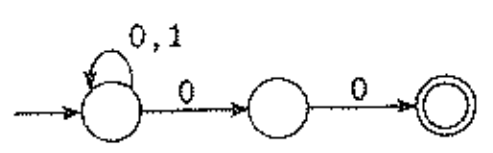
\includegraphics[width=0.3\textwidth]{images/ex-automi1.PNG}
    %\captionof{figure}{Diagramma di stato per un automa finito $M_2$}
\end{minipage}
\end{Exercise}

\begin{Exercise}{}{}
\textit{Sia $r=1^*(001^+)^*$, dove $+$ significa "almeno un'occorrenza". Costruire un DFA tale che $L(D)=L(r)$ con 3 stati e alfabeto $\{0,1\}$.}

\begin{minipage}{\textwidth}
    \centering
    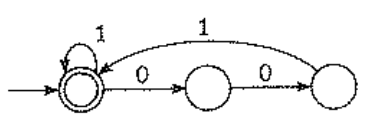
\includegraphics[width=0.3\textwidth]{images/ex-automi2.PNG}
    %\captionof{figure}{Diagramma di stato per un automa finito $M_2$}
\end{minipage}
\end{Exercise}

\begin{Exercise}{}{}
\textit{Data l’espressione regolare $R = (01^+)^*$, costruire il DFA $D$ tale che $L(D) = \{w\in \{0, 1\}^*| w\notin L(R)\}$.}

Prima di tutto, costruiamo un DFA $D_R$ tale che $L(D_R) = L(R)$.

\begin{minipage}{\textwidth}
    \centering
    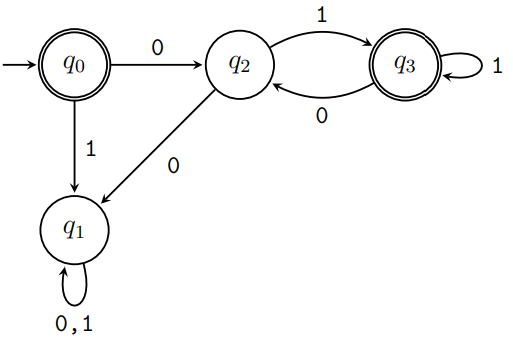
\includegraphics[width=0.37\textwidth]{images/ex-automi3.1.PNG}
    %\captionof{figure}{Diagramma di stato per un automa finito $M_2$}
\end{minipage}

A questo punto, ci basta costruire il DFA $D$ tale che $L(D) = \overline{L(D_R)}$ utilizzando la
chiusura del complemento in REG.

\begin{minipage}{\textwidth}
    \centering
    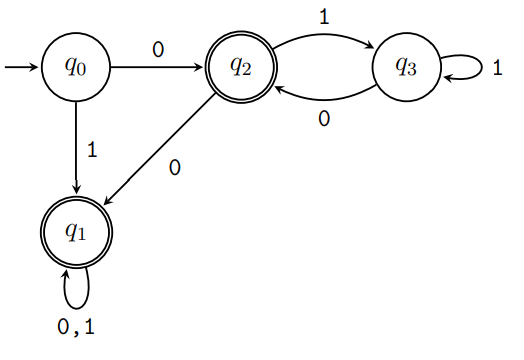
\includegraphics[width=0.37\textwidth]{images/ex-automi3.2.PNG}
    %\captionof{figure}{Diagramma di stato per un automa finito $M_2$}
\end{minipage}
\end{Exercise}

\begin{Exercise}{}{}
\textit{Dato il linguaggio $L = \{w\in \{0, 1\}^*: |w|_0 = |w|_1\}$, dimostrare che $L$ non è regolare.}

\begin{demonstration}
Supponiamo per assurdo che $L$ sia regolare, implicando che per esso debba valere il
pumping lemma, dove $p$ è la lunghezza del pumping. 

Consideriamo quindi la stringa $w = 0^p1^p\in L$. Poiché $|w|\geq p$, possiamo suddividerla in tre sottostringhe $x, y, z\in\Sigma^*$ tali che $w = xyz$. Poiché la terza condizione del pumping lemma impone che $|xy|\leq p$ e poiché $w := 0^p1^p$, ne segue che $xy = 0^m$ e $z = 0^{p-m}1^p$, dove $m\in [1, p]$. Inoltre, per la seconda condizione, si ha che $|y| > 0$, dunque necessariamente si ha che $x = 0^{m-k}$ e $y = 0^k$, dove $k\in [1, m]$. A questo punto, consideriamo la stringa $xy^0z$. Notiamo immediatamente che 
\begin{equation*}
xy^0z = 0^{m-k}(0^k)^00^{p-m}1^p = 0^{m-k}0^{p-m}1^p = 0^{p-k}1^p\implies |xy^0z|_0\neq|xy^0z|_1\implies xy^0z\notin L    
\end{equation*}
contraddicendo la prima condizione del lemma per cui si ha che $\forall i\geq0, xy^iz\in L$. Dunque, ne segue necessariamente che $L$ non sia regolare.
\end{demonstration}
\end{Exercise}

\begin{Exercise}{}{}
\textit{Dato il linguaggio $L = \{1^{n^2}| n\geq0\}$, dimostrare che $L$ non è regolare.}

\begin{demonstration}
Supponiamo per assurdo che $L$ sia regolare, implicando che per esso debba valere il
pumping lemma, dove $p$ è la lunghezza del pumping. 

Consideriamo quindi la stringa $w := 1^{p^2}\in L$. Poiché $|w|\geq p$, possiamo suddividerla in tre sottostringhe $x, y, z\in\Sigma^*$ tali che $w = xyz$. Poiché la terza condizione del lemma impone che $|xy| \leq p$ e poiché $w := 1^{p^2}$, ne segue che $xy = 1^m$ e $z = 1^{p^2-m}$, dove $m\in [1, p]$. Inoltre, per la seconda condizione del lemma, si ha che $|y| > 0$, dunque necessariamente si ha che $x = 1^{m-k}$ e $y = 1^k$, dove $k\in [1, m]$. A questo punto, consideriamo la stringa $xy^0z$. Notiamo immediatamente che 
\begin{equation*}
xy^0z = 1^{m-k}(1^k)^01^{p^2-m} = 1^{p^2-k}   
\end{equation*}
Tuttavia, poiché $k\in [1, p]$, ne segue che $\nexists n \geq0| n^2 = p^2 - k$, implicando dunque che $xy^0z\notin L$, contraddicendo la prima condizione del lemma per cui si ha che $\forall i \geq0xy^iz\in L$. Dunque, ne segue necessariamente che $L$ non sia regolare.
\end{demonstration}
\end{Exercise}